\section{Verschiedene Clients}
Um einen Client f\"ur diese Anwendung zu schreiben existieren viele verschiedene M\"oglichkeiten. Die folgenden vier Varianten sollen die Vielfältigkeit und Flexibilität der Implementierung zeigen.\\
Jedem Client dieser Anwendung werden ausschlie\ss lich die vorher festgelegten Funktionalit\"aten des \courier{Controllers} zur Verf\"ugung gestellt. Diese Auswahl wird \"uber eine Schnittstelle mit dem Namen \courier{MBeanController} angeboten. Um einen Zugriff auf die bereitgestellten Operationen zu erhalten, muss sich ein Client zun\"achst am MBean-Server anmelden. Eine Anmeldung kann lokal oder \"uber die Remote Method Invocation geschehen. Nach der Anmeldung sind die spezifizierten Methoden \"uber den \courier{MBeanController} ausf\"uhrbar.

\begin{itemize}
	\item JConsole: Die einfachste Variante eine Verbindung aufzubauen bietet die JConsole. Dies ist ein grafisches Monitoring-Tool welches es ermöglicht, lokale und auch entfernte Anwendungen zu \"uberwachen. Es bietet zus\"atzlich eine Vielzahl an n\"utzlichen Messwerten wie Speicherverbrauch oder CPU-Auslastung.
	
%\begin{figure}[!htb]
%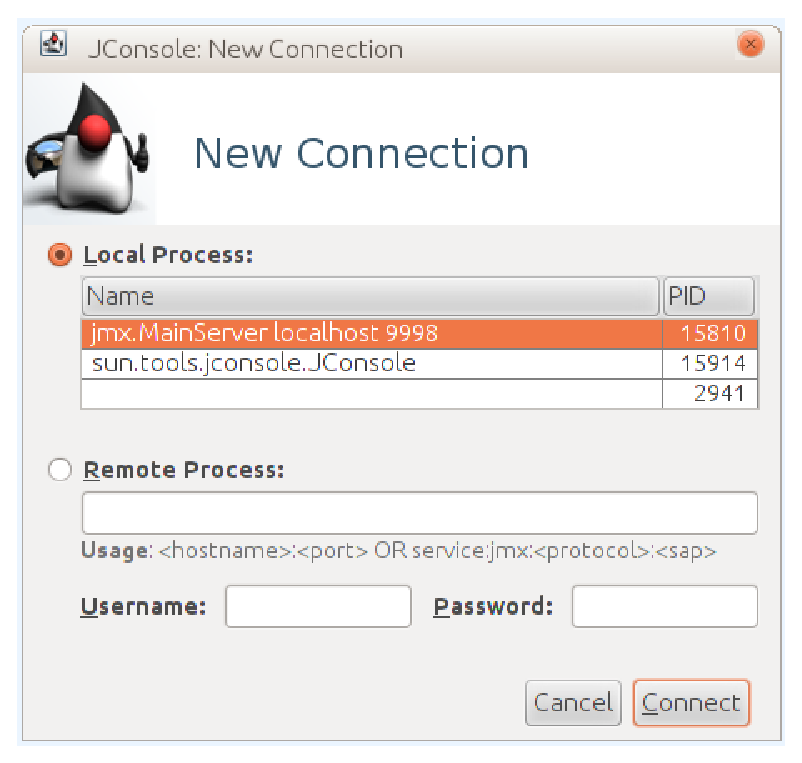
\includegraphics[scale=0.6]{graphics/jConsole.eps}
%\centering
% \caption[JConsole MBeans]{JConsole Angemeldete MBeans}
% \label{fig:JConsole}
%\end{figure}
%
%\begin{figure}[!htb]
%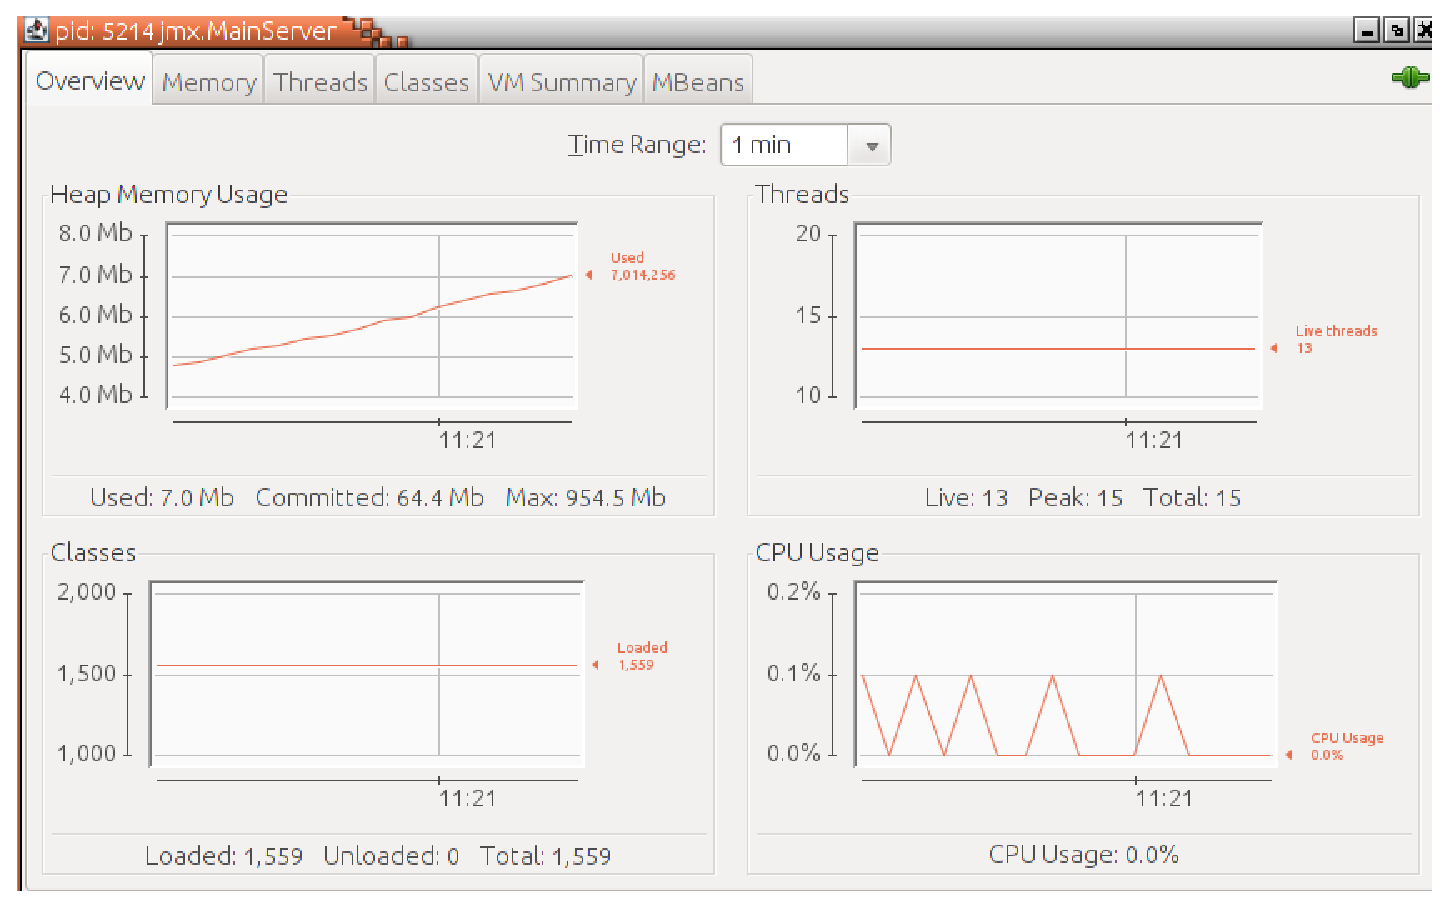
\includegraphics[scale=0.5]{graphics/jConsole2.eps}
%\centering
% \caption[JConsole Monitoring]{JConsole Monitoring}
% \label{fig:JConsole2}
%\end{figure}	
	
	\item Shell-Script: Eine andere Möglichkeit, um beispielsweise einen konsolenbasierten Client zu schrieben, ist durch die Verwendung von jmxterm\footnote{http://wiki.cyclopsgroup.org/jmxterm} gegeben. Daf\"ur ist lediglich ein einfaches Skript f\"ur den Verbindungsaufbau zum MBeanServer und der \"Ubergabe einer Ausf\"uhrungsliste notwendig. Die gew\"unschten Interaktionen werden unter Ber\"ucksichtigung einer gewissen Syntax in diese Liste\footnote{einfache Textdatei} geschrieben und dem Skript als Parameter \"ubergeben. Ein konkretes Beispiel wird im Kapitel Implementierung aufgezeigt.	
	
	\item Webbrowser: F\"ur die Agent-View \"uber einen Webbrowser bietet sich die Nutzung von JMXTools an. Neben dem MBeanServer muss die durch die Library bereitgestellte Klasse \courier{HtmlAdaptorServer} gestartet werden. Dieser wird zusätzlich ein Host und ein Port \"ubergeben. Mittels Webbrowser kann nun über den Host und den Port eine Verbindung zum \courier{MBeanServer} aufgebaut werden. Anschlie\ss end stehen die \courier{MBeans} zur Auswahl bereit. Die Operationen des gewählten \courier{MBeans} lassen sich nun \"uber den Webbrowser steuern.
	
%\begin{figure}[!htb]
%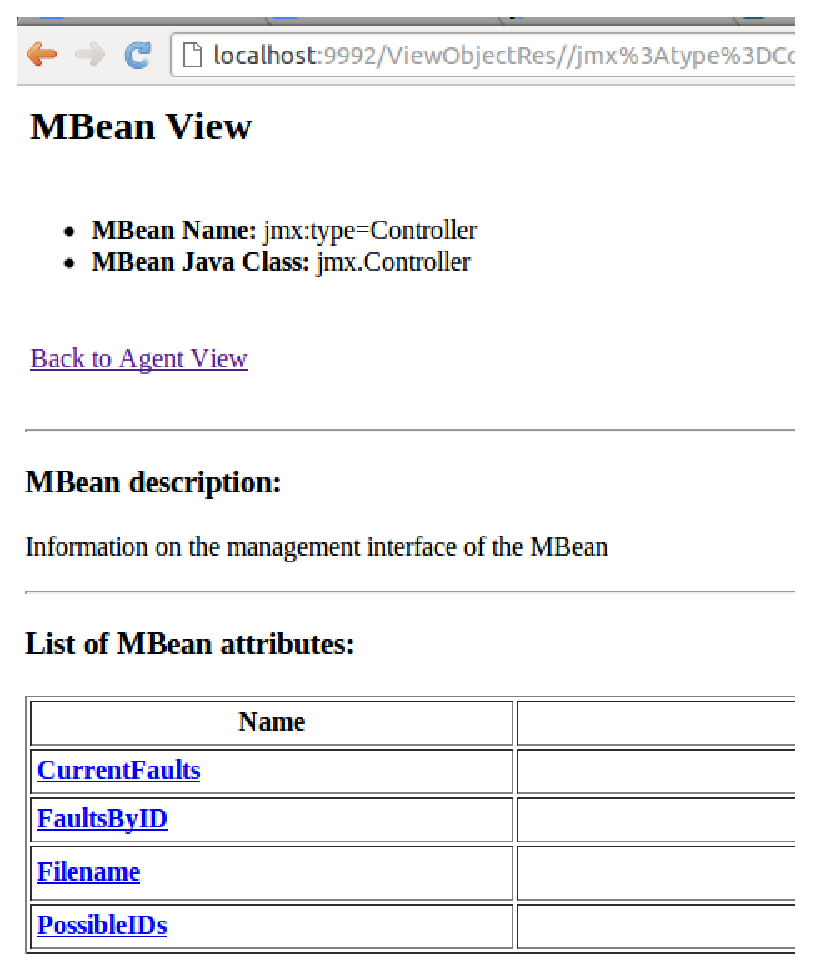
\includegraphics[scale=0.7]{graphics/htmlView.eps}
%\centering
% \caption[HtmlAdaptorServer]{HtmlAdaptorServer}
% \label{fig:HtmlAdaptorServer}
%\end{figure}		
	
	\item Java-Client: Java-Clients lassen sich ebenfalls über die \courier{ControllerMBean} Schnittstelle sehr leicht integrieren. Die Verbindung zum \courier{MBeanServer} wird \"uber RMI oder lokal aufgebaut. Ist die Verbindung erfolgreich können Variablen über \courier{Attribut}-Objekte gesetzt oder erfragt werden. Um die Methoden auszuführen ist ein \courier{Connection}-Objekt erforderlich.
\end{itemize}


